\chapter{Aquecimento Global e Eletricidade}
\localtableofcontents 

Este capítulo é baseado nas notas de aula do curso, ministrado em 17/08/2023, e no capítulo 24 de \textcite{cretì_fontini_2019}.

\section{Preço de Carbono e Mercados de Eletricidade}
Uma das formas que os economistas encontraram para ajudar a mitigar o problema do aquecimento global é precificar o carbono emitido na produção dos bens - inclusive eletricidade. Essa prática é intuitiva do ponto de vista econômico, pois a emissão de gases poluentes configura uma externalidade negativa - e a teoria microeconômica diz que existe um preço ótimo da externalidade tal que faça o problema descentralizado convergir para o problema do planejador central.

Na prática, existem algumas formas de se construir esse mercado de carbono. Uma delas é dar às empresas licenças para emissões proporcionalmente às suas emissões históricas, por exemplo, e permitir que elas comercializem com as demais por mais licenças a fim de expandir as emissões. Independente do sistema de como se dão as licenças, o processo de distribuí-las gratuitamente é chamado de "\textbf{apadrinhamento}" (em contraponto à um leilão, por exemplo).

Nesse sistema, o lucro das firmas irá subir sempre, pois elas conseguem reverter 100\% do aumento de custos para o consumidor. Isso se dá pois o custo marginal de produção se mantém constante, mas o custo-oportunidade de geração aumenta, pois as firmas podem vender as licenças no mercado. Graficamente, haverá um deslocamento da curva de oferta para a esquerda, tal qual exemplificado na Figura~\ref{fig:gdfth}.

\begin{figure}
    \centering
    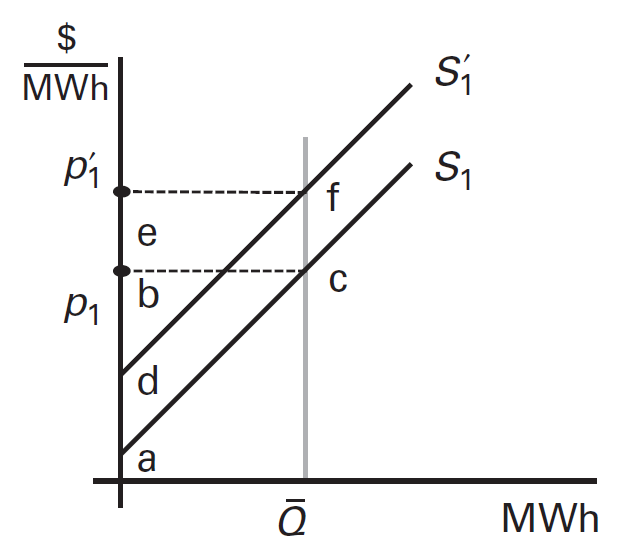
\includegraphics[scale=.25]{figure/grandfather.png}
    \caption{Consequências do Apadrinhamento}
    \label{fig:gdfth}
\end{figure}

Entretanto, caso as licenças tivessem sido vendidas em um leilão, obtê-las muda diretamente o custo marginal das firmas - podendo ou não, portanto, alterar a ordem de mérito. Caso não haja nenhuma mudança na ordem de mérito, as conclusões serão as mesmas do caso de apadrinhamento i.e. haverá \textit{pass-through} completo para o consumidor. Caso a ordem mude, contudo, então haverá \textit{pass-through} parcial, apenas. Isso pode ser visto graficamente na Figura~\ref{fig:cc}, onde a existência das licenças faz com que o aumento do preço marginal do sistema seja menor que o aumento no custo marginal da firma marginal - i.e. não há \textit{pass-through} completo.

\begin{figure}
    \centering
    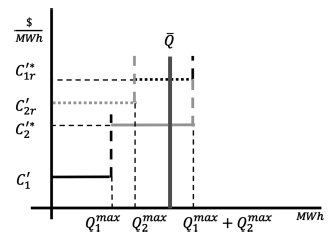
\includegraphics[scale=.6]{figure/cc_meritorder.png}
    \caption{Mudança na Ordem de Mérito}
    \label{fig:cc}
\end{figure}